\documentclass{beamer}

\usepackage{stacks} % custom commands for typesetting stacks

\usepackage{listings,bold-extra}
\lstset{basicstyle=\ttfamily,
        mathescape=true,
        keepspaces=false,
        morekeywords={:=,+,-,*,/,goto,if,<,<=,>,>=,=}}
\usepackage{tikz}
\usetikzlibrary{shapes.misc}

\usepackage{../lib/minted}
\usemintedstyle{bw}
\newminted{factor}{gobble=0,frame=none}
\newmint{factor}{}

\mode<presentation>{
  \usetheme{CambridgeUS}
  \useoutertheme{infolines}
  \setbeamertemplate{navigation symbols}{}
  \AtBeginSection[]{\frame{\tableofcontents[currentsection]}}
}

\title{Global Value Numbering in Factor}
\author{Alex Vondrak}
\institute{\texttt{ajvondrak@csupomona.edu}}
\date{September 1, 2011}
\pgfdeclareimage[width=0.5\textwidth]{logo}{dependencies.png}
\titlegraphic{\pgfuseimage{logo}}

\begin{document}

\maketitle

\begin{frame}{Factor}
  Factor (\url{http://factorcode.org/})
  \begin{itemize}
    \item Started development September 2003---a baby among languages
    \item \alert{Stack-based}
    \item Object-oriented
    \item Dynamically typed
    \item Extensive standard library
    \item High-level, yet fully \alert{compiled}
  \end{itemize}

  Won't really have time to discuss the language in depth
\end{frame}

\begin{frame}[fragile]{Stacks as an Evaluation Model}
  \begin{example}[Code]
    \begin{verbatim}
1 2 +
    \end{verbatim}
  \end{example}

  \begin{example}[Execution]
    \begin{columns}[c,onlytextwidth]
      \begin{column}[c]{.5\textwidth}
        \begin{verbatim}
push(1);
push(2);
y = pop();   // y = 2;
x = pop();   // x = 1;
push(x + y); // push(3);
        \end{verbatim}
      \end{column}

      \begin{column}[c]{.5\textwidth}
        \stackop{3}{+}{1 2 ~}{3 ~}
      \end{column}
    \end{columns}
  \end{example}
\end{frame}

\section{Compiler}

\subsection{Structure}

\begin{frame}{Organization}
  Non-optimizing base compiler
  \begin{itemize}
    \item VM written in C++
    \item Responsible for basic runtime services
    \begin{itemize}
      \item Garbage collection
      \item Method dispatch
      \item Polymorphic inline caches
      \item \ldots
    \end{itemize}
    \item Single pass---outputs assembly stubs for primitives
  \end{itemize}

  \alert{Optimizing compiler}
  \begin{itemize}
    \item Written in Factor code
    \begin{itemize}
      \item Possible by \emph{bootstrapping}
    \end{itemize}
    \item Optimizes in passes across two \alert{intermediate representations}
    (IRs)
    \begin{itemize}
      \item High-level IR (\texttt{compiler.tree})
      \item Low-level IR (\texttt{compiler.cfg})
    \end{itemize}
  \end{itemize}
\end{frame}

\begin{frame}{High-level IR}
  \begin{itemize}
    \item Tree of \texttt{node} objects
    \item Very simple virtual instruction set
    \begin{itemize}
      \item \texttt{\#introduce}, \texttt{\#return}
      \item \texttt{\#push} \& \texttt{\#call}
      \item \texttt{\#renaming}---\texttt{\#copy} \& \texttt{\#shuffle}
      \item \texttt{\#declare} \& \texttt{\#terminate}
      \item \texttt{\#branch}---\texttt{\#if} \& \texttt{\#dispatch}
      \item \texttt{\#phi}
      \item \texttt{\#recursive}, \texttt{\#enter-recursive},
            \texttt{\#call-recursive}, \texttt{\#return-recursive}
      \item \texttt{\#alien-node}, \texttt{\#alien-invoke},
            \texttt{\#alien-indirect}, \texttt{\#alien-assembly},
            \texttt{\#alien-callback}
    \end{itemize}
    \item Input/output values of stack given unique names
  \end{itemize}
\end{frame}

\begin{frame}[fragile]{High-level IR}{\texttt{1~2~+}}
  \begin{example}
    \begin{verbatim}
V{
    T{ #push { literal 1 } { out-d { 6256273 } } }
    T{ #push { literal 2 } { out-d { 6256274 } } }
    T{ #call
        { word + }
        { in-d V{ 6256274 6256273 } }
        { out-d { 6256275 } }
    }
    T{ #return { in-d V{ 6256275 } } }
}
    \end{verbatim}
  \end{example}
\end{frame}

\begin{frame}[fragile]{Low-level IR}
  \begin{itemize}
    \item Control flow graph (CFG)
    \begin{itemize}
      \item Basic blocks = maximal sequence of ``straight-line'' code
      \item Directed edges = transfer of control flow
    \end{itemize}
    \item \texttt{insn} objects modeled closely after assembly-like
          instructions
    \item \alert{Static single assignment} (SSA) form
  \end{itemize}
  \begin{onlyenv}<1>
  \begin{center}
    \begin{minipage}{0.4\linewidth}
      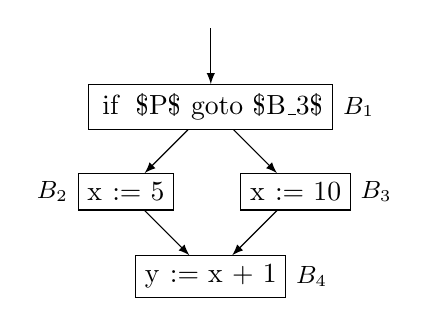
\begin{tikzpicture}[node distance=0.6in,>=latex]
      \node[draw,label=right:{\small $B_1$}] (1) at (0,-1)
        {\lstinline|if $P$ goto $B_3$|};
      \node[draw,label=left:{\small $B_2$}] (2) [below left of=1]
        {\lstinline|x := 5|};
      \node[draw,label=right:{\small $B_3$}] (3) [below right of=1]
        {\lstinline|x := 10|};
      \node[draw,label=right:{\small $B_4$}] (4) [below right of=2]
        {\lstinline|y := x + 1|};

      \draw[->] (0,0) -- (1);
      \draw (1) edge[->] (2)
                edge[->] (3)
            (2) edge[->] (4)
            (3) edge[->] (4);
      \end{tikzpicture}
    \end{minipage}
    \vrule
    \begin{minipage}{0.4\linewidth}
      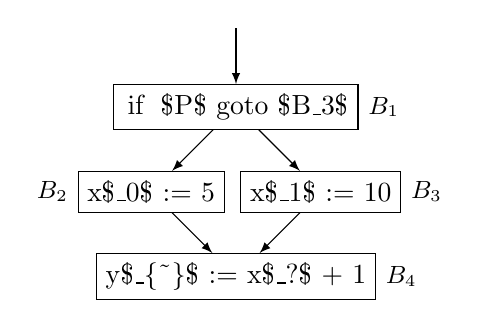
\begin{tikzpicture}[node distance=0.6in,>=latex]
      \node[draw,label=right:{\small $B_1$}] (1) at (0,-1)
        {\lstinline|if $P$ goto $B_3$|};
      \node[draw,label=left:{\small $B_2$}] (2) [below left of=1]
        {\lstinline|x$_0$ := 5|};
      \node[draw,label=right:{\small $B_3$}] (3) [below right of=1]
        {\lstinline|x$_1$ := 10|};
      \node[draw,label=right:{\small $B_4$}] (4) [below right of=2]
        {\lstinline|y$_{~}$ := x$_?$ + 1|};

      \draw[->] (0,0) -- (1);
      \draw (1) edge[->] (2)
                edge[->] (3)
            (2) edge[->] (4)
            (3) edge[->] (4);
      \end{tikzpicture}
    \end{minipage}
  \end{center}
  \end{onlyenv}
  \begin{onlyenv}<2>
  \begin{center}
  \begin{tikzpicture}[node distance=0.7in,>=latex]
  \node[draw,label=right:$B_1$] (1) at (0,-1) {\lstinline|if $P$ goto $B_3$|};
  \node[draw,label=left:$B_2$] (2) [below left of=1] {\lstinline|x$_0$ := 5|};
  \node[draw,label=right:$B_3$] (3) [below right of=1] {\lstinline|x$_1$ := 10|};
  \node[draw,label=right:$B_4$] (4) [below right of=2] {
  \begin{lstlisting}
x$_2$ := $\phi$(x$_0$,x$_1$)
y$_{~}$ := x$_2$ + 1
  \end{lstlisting}
  };

  \draw[->] (0,0) -- (1);
  \draw (1) edge[->] (2)
            edge[->] (3)
        (2) edge[->] (4)
        (3) edge[->] (4);
  \end{tikzpicture}
  \end{center}
  \end{onlyenv}
\end{frame}

\subsection{Optimizations}

\begin{frame}[fragile]{Optimizations---High-level IR}
\footnotesize
\begin{center}
\begin{minipage}{0.5\linewidth}
\begin{Verbatim}[commandchars=\\\{\}]
\PY{k}{:} \PY{n+nf}{optimize-tree} \PY{n+nf}{(} \PY{n+nv}{nodes} \PY{n+nf}{--} \PY{n+nv}{nodes'} \PY{n+nf}{)}
  [
      analyze-recursive
      normalize
      propagate
      cleanup
      \PY{k}{dup }run-escape-analysis? [
          escape-analysis
          unbox-tuples
      ] \PY{k}{when}
      apply-identities
      compute-def-use
      remove-dead-code
      ?check
      compute-def-use
      optimize-modular-arithmetic
      finalize
  ] \PY{k}{with-scope ;}
\end{Verbatim}
\end{minipage}
\end{center}
\end{frame}

\begin{frame}[fragile]{Optimizations---Low-level IR}
  \renewcommand{\theFancyVerbLine}{%
    \ifnum\value{FancyVerbLine}=9%
    $\longrightarrow$\else{}\fi}
  \begin{center}
  \begin{minipage}{0.5\linewidth}
  \begin{factorcode*}{linenos}
: optimize-cfg ( cfg -- cfg' )
    optimize-tail-calls
    delete-useless-conditionals
    split-branches
    join-blocks
    normalize-height
    construct-ssa
    alias-analysis
    value-numbering
    copy-propagation
    eliminate-dead-code ;
  \end{factorcode*}
  \end{minipage}
  \end{center}
\end{frame}

\section{Value Numbering}

\section{Results}

\end{document}
